\documentclass[a4paper]{report}

\usepackage{natbib} % Required to change bibliography style to APA
\usepackage{amsmath} % Required for some math elements 
\usepackage{hyperref}

\usepackage{epsfig}            % to insert PostScript figures
\graphicspath{ 
  {figures/} 
}

%Change figure names
\renewcommand{\figurename}{Fig}

\usepackage[bf,footnotesize]{caption} % make captions small and label bold

\addtocounter{chapter}{1} %Because starting at zero is silly
\makeatletter
\renewcommand{\thesection}{\@arabic\c@section}
\renewcommand{\thefigure}{\@arabic\c@figure}
\makeatother

\setlength\parindent{0pt} % Removes all indentation from paragraphs

%\title{Spatial two-alternative forced-choice probabilistic switching task} % Title
%\author{John \textsc{Smith}} % Author name
%\date{\today} % Date for the report

\begin{document}

%\maketitle % Insert the title, author and date

%set the number of sectioning levels 
\setcounter{secnumdepth}{2}

\begin{center}
\textbf{\Large{Spatial two-alternative forced-choice probabilistic switching task}}
\end{center}

% \begin{abstract}
% Abstract text
% \end{abstract}


\subsection*{The Task}

This task is designed to test how animals change their behavior according to the value of different actions in different contexts. We manipulate the reward probability of the two possible choices and test whether animals adapt their behavior accordingly.
Mice are placed in a 3-port behavior box. Each port can detect a poke and deliver water. The task is organized in blocks of random size (from 7-23 trials). In each block, one port is rewarded 75\% of the time, the other is not rewarded. Animals must poke in the center port and then either poke in the left port or in the right port.

\subsubsection{Details:} 
\begin{itemize}
\item It is useful to require the center port to last at least 200ms to avoid 'false pokes'.
\end{itemize}


\subsection*{Behavior Day 1: Implementation day}

\begin{enumerate}
\item Design the state matrix
\item Assemble the hardware (ports, valves, etc...)
\item Code the task for Bpod (use guide code)
\item Try the task yourself
\item Try the task with a mouse
\end{enumerate}


\subsection*{Behavior Day 2: Behavioral session}
\begin{enumerate}
\item Run a behavioral session
\item Plot the fraction of left choices as function of trials relative to block switch (Fig 1b).
\item Plot the fraction of switches as a function of reward history in previous 2 trials (Fig 1c).
\item Fit regression model for past history (Fig 2a)
\item Plot fraction of left choices vs predicted fraction of left choices (Fig. 2c)
\end{enumerate}

\subsection*{Behavior Day 3:}
\begin{enumerate}
\item Record from a behaving animal
\item Plot PSTH's for right/left, correct/incorrect trials
\item Compare firing at beginning vs end of blocks
\item Plot firing as function of subjective poke value based on regression model
\end{enumerate}


\subsection*{Useful references}
\begin{itemize}
\item Tai et al Nat Neuro 2012 (attached)
\item Bpod wiki \url{sites.google.com/site/bpoddocumentation/}
\item Bcontrol documentation \url{brodywiki.princeton.edu/bcontrol/index.php/RealTime_Linux_State_Machine}
\end{itemize}


\subsection*{Appendix}

\subsubsection{Psychometric function}

Psychometric functions (PF) relate the behavior on a given task to some physical characteristic of the stimulus (fraction of correct trials vs contrast). Typically, PF's are measured to determine parameters that summarize the behavior of the subject. In order to do that, some continuous function has to be fitted to the experimental measurement. The logistic function is one of a variety of functions that can be used for this purpose. Other functions that are also used to fit psychometric measurements are the Cumulative Normal (if one assumes sensory noise to be normal) or the Weibull function.

\subsubsection{Logistic function:}

\begin{equation*}
p=\frac{1}{1+e^{-\alpha(x-\beta)}}
\end{equation*}

Two parameters describe the logistic function: the slope ($\alpha$) and the bias ($\beta$). Other parameters that are of interest are the standard error of these two quantities and some measure of the goodness-of-fit of the model itself. The logistic function can also be extended to account for lapses or guesses:

\begin{equation*}
p=\gamma + \frac{1-\gamma-\lambda}{1+e^{-\alpha(x-\beta)}}
\end{equation*}


\subsubsection*{Fitting}

The most common method to fit logistic functions is through Maximum Likelihood. In MATLAB, this can be done using \texttt{glmfit}. All is needed is a predictor matrix $X$ and a vector $y$ of observed responses. Because the logistic regression is a special case of a generalized linear model, we also need to specify the binomial distribution and the logit link.

\begin{verbatim}
	[b,dev] = glmfit(X,y,'binomial','logit');
\end{verbatim}

To evaluate the model we can use glmval

\begin{verbatim}
	y_p = glmval(b,X_p,'logit');
\end{verbatim}

\subsubsection*{Estimating confidence intervals and goodness-of-fit:}

The MATLAB function glmfit also returns useful quantities to evaluate the goodness-of-fit of the model and interval of confidence for predictions derived from the model.

\begin{verbatim}
	[b,dev,stats] = glmfit(X,y,'binomial','logit');
\end{verbatim}

The variable dev is the deviance, which is a generalization of the residual sum of squares. This can be useful to perform tests between different models and test weather including more terms to the predictor matrix gives a significantly better model. The stat variable is a structure with several useful statistical measures of the model: confidence intervals for the weights, p-values, residuals, etc. This can be used to get error bars for the predictions of the model:

\begin{verbatim}
	[prediction,dlo,dhi] = glmval(b,X_p,'logit',stats,.95,100);
\end{verbatim}

Another useful way to estimate the error on the weights of the logistic regression is to perform a 'bootstrap analysis'. The basic idea is to produce a large number of artificial data sets originating from the real data and recompute the fit for every one of them. The result will be a distribution of α's and β's whose standard deviation is an estimate of their measurement error.

\subsubsection*{Finite State Machine}

A useful way to represent behavioral tasks is by finite state machines (FSM). Also, implementing tasks in Bpod uses this same representation. FSM's consist of a fixed number of states, inputs and outputs. The inputs cause transitions between states (e.g. the detection of a poke) and the outputs are used to control some actuator (e.g. opening a water valve). Another useful property of states are timers. Each state has an internal clock which will be triggered the moment the FSM enters to that state. A 'time is up' event, associated with that timer, can be defined such that when the timer reaches a specified time, an internal signal will be generated. That signal can be used to generate a transition between states.


\begin{figure}[h]
\center
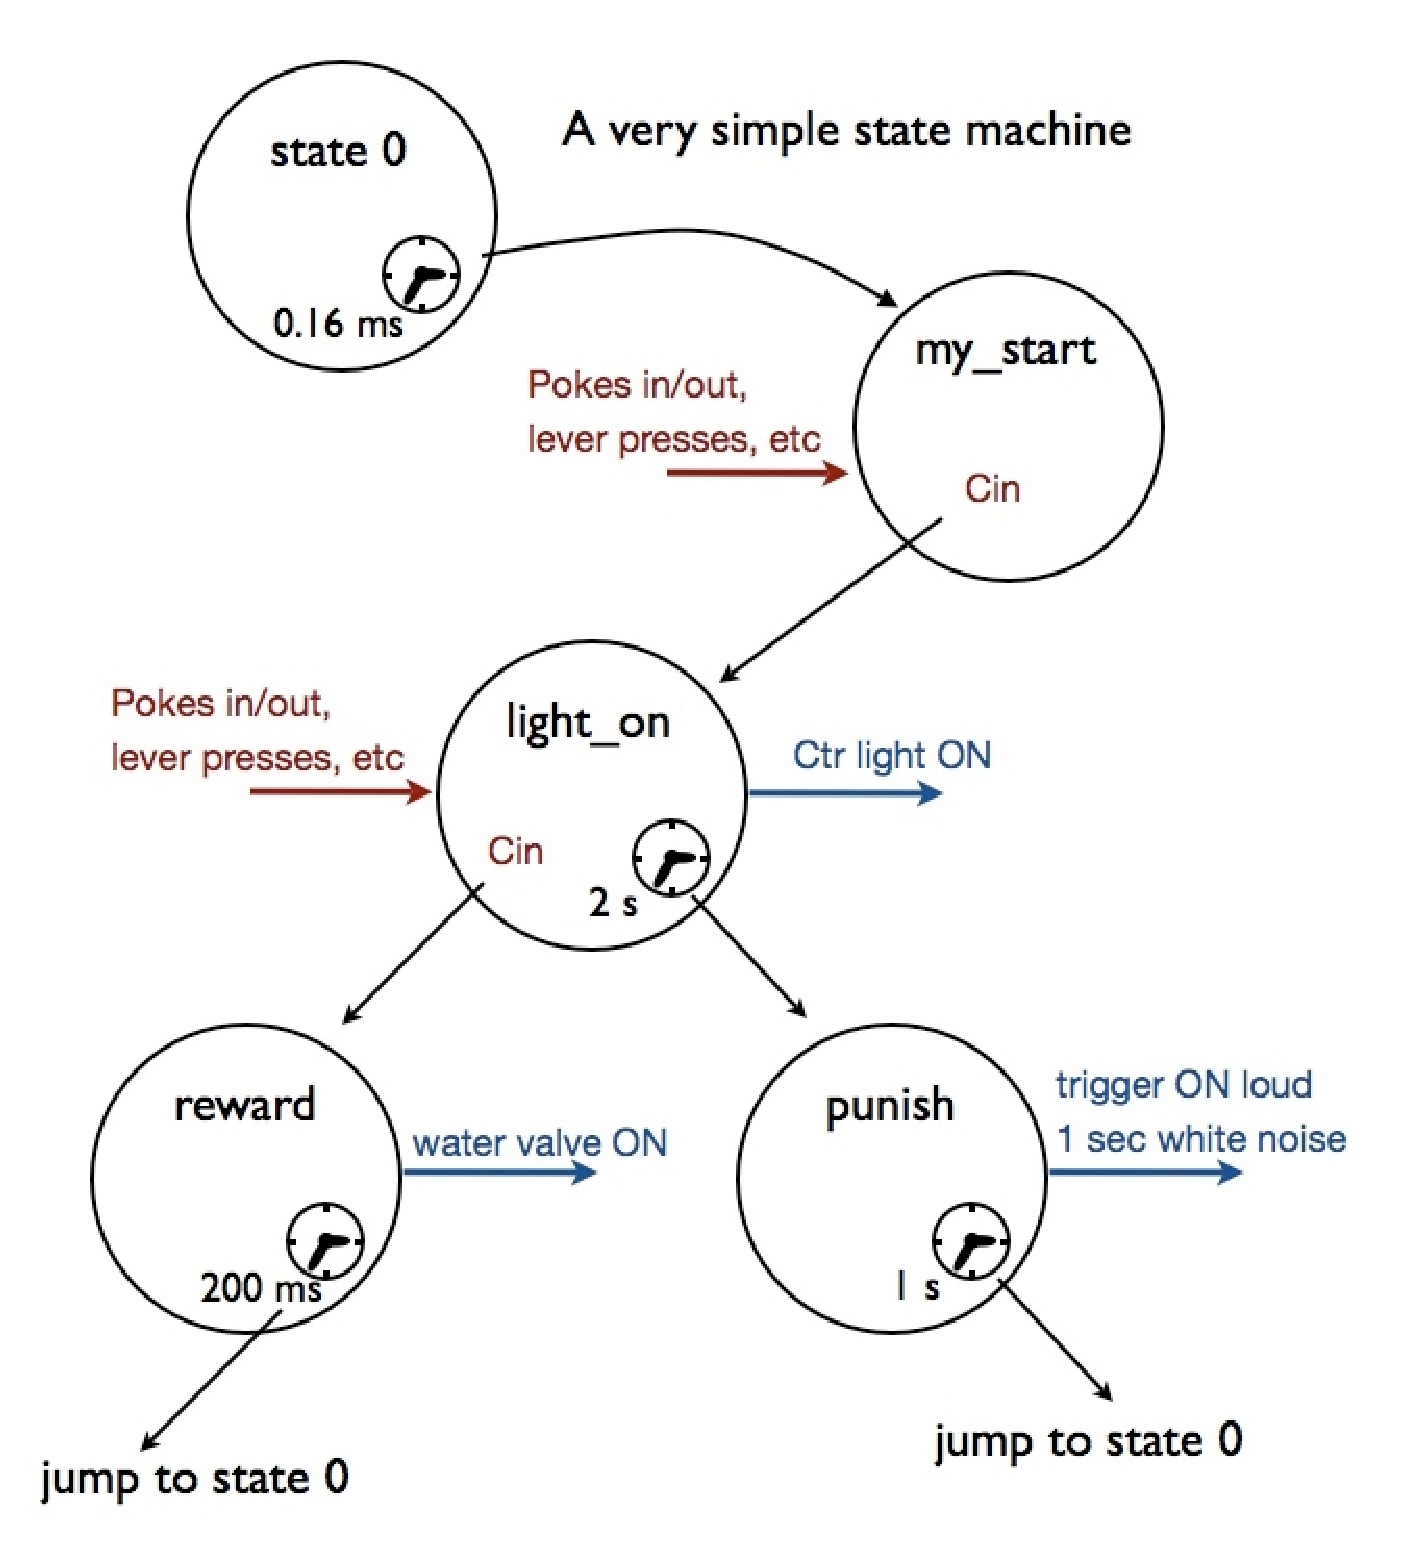
\includegraphics[width=3in]{figure/SimplestFST.eps}
\caption{A very simple state machine. From Bcontrol documentation (Brody lab)}
\end{figure}

\end{document}
